% Created 2017-08-22 Ter 20:21
\documentclass[11pt]{article}
\usepackage[utf8]{inputenc}
\usepackage[T1]{fontenc}
\usepackage{fixltx2e}
\usepackage{graphicx}
\usepackage{longtable}
\usepackage{float}
\usepackage{wrapfig}
\usepackage{rotating}
\usepackage[normalem]{ulem}
\usepackage{amsmath}
\usepackage{textcomp}
\usepackage{marvosym}
\usepackage{wasysym}
\usepackage{amssymb}
\usepackage{hyperref}
\tolerance=1000
\usepackage[margin=3cm]{geometry}
\author{Cecília Carneiro e Silva}
\date{23/08/2017}
\title{Trabalho 02 - Ag simple}
\hypersetup{
  pdfkeywords={},
  pdfsubject={},
  pdfcreator={Emacs 25.1.1 (Org mode 8.2.10)}}
\begin{document}

\maketitle

\section{Ag - Simple Example}
\label{sec-1}

Implementação de um exemplo de Algoritmo Genético. Seguindo a seção 3 do artigo do Tomassini. A linguagem utilizada foi Racket Language. Repositório da aplicação: \url{https://github.com/ceciliacsilva/agSimple}.
Minimização da função f(x), deseja-se encontrar o valor de x para f(x) mínimo.

\subsection{Considerações}
\label{sec-1-1}

\begin{itemize}
\item Avaliação dos indivíduos: baseada na função de aptidão (fitness), indica a qualidade do indivíduo na população.
\item Para o resultado da função aptidão ser positivo, sendo f(x) negativa para todo x, criou-se g(x) = - f(x).
\item Na verdade, foi encontrado o valor máximo da função.
\item Critérios de parada: número máximo de gerações, repetição do melhor indivíduo por n gerações.
\end{itemize}

\subsection{Estruturação}
\label{sec-1-2}

\begin{itemize}
\item Cromossomo = string, "0011011001"
\item Indivíduo = pair, '(cromossomo . fitness)
\item População = list, '((cromossomo1 . fitness1) (cromossomo2 . fitness2) \ldots{})
\end{itemize}

\subsection{Parametros do AG}
\label{sec-1-3}

\begin{itemize}
\item pc: 0,6 (artigo)
\item pm: 0,01 (artigo)
\item tamanho da população: 50 (artigo)
\item x máximo: 512 (artigo)
\item cromossomo máximo: 1024 (artigo)
\item número máximo de gerações: 200
\item repetição máxima do melhor indivíduo: 5
\end{itemize}

\subsection{Resultados}
\label{sec-1-4}

\begin{verbatim}
> ;;(find-min <nome_simulacao> <parametros-ag>)
> (find-min "simul3" *ag*)
x para f(x) mínimo: 421 valor: 418.9827640161443
'("1101001010" . 418.9827640161443)
\end{verbatim}

Gráficos exibidos ao fim da execução:

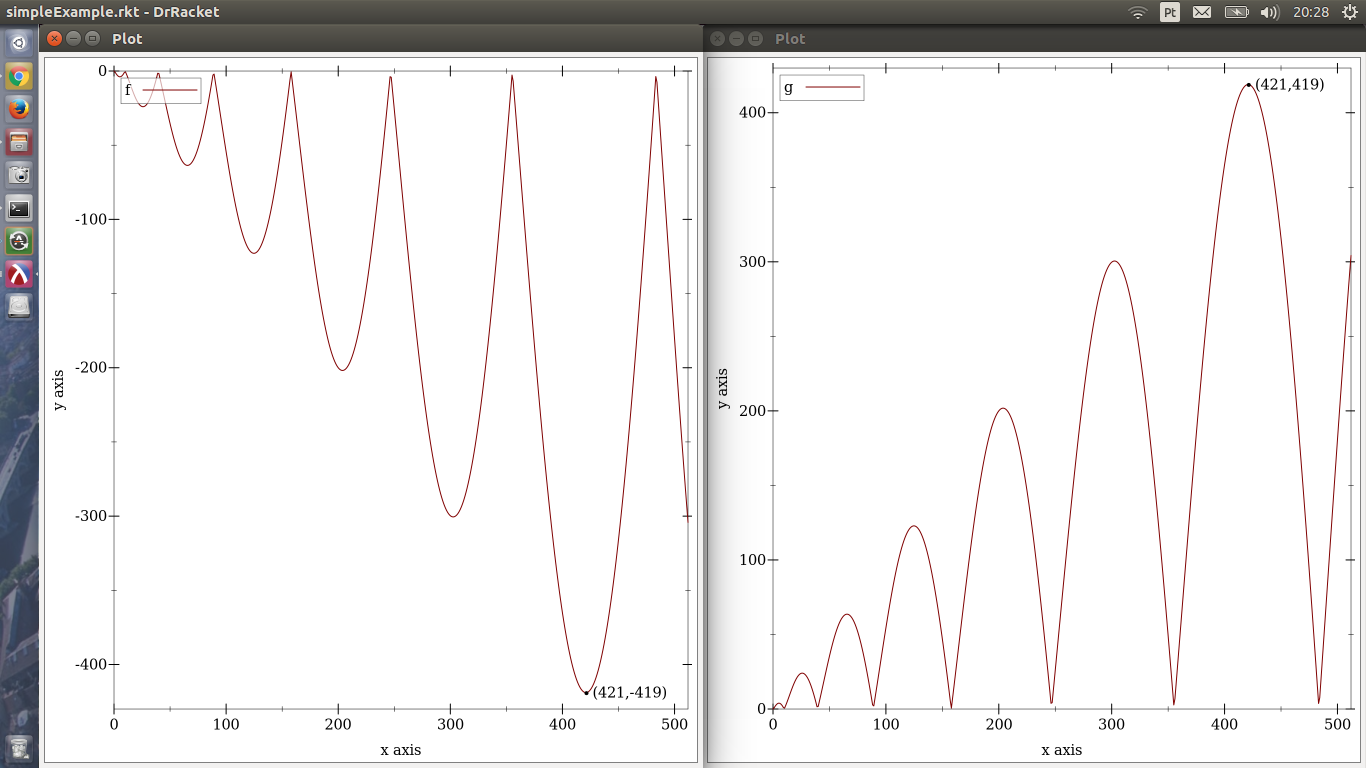
\includegraphics[width=.9\linewidth]{imagens/ag-fgs3.png}

Vídeo com a evolução da população: \url{https://github.com/ceciliacsilva/agSimple/blob/master/simul3/output.mp4}

\begin{itemize}
\item OBS: para gerar o vídeo é necessário entrar o diretório <nome$_{\text{simulacao}}$> e executar o script "toVideo.sh".
\end{itemize}

\begin{verbatim}
$ cd <nome_simulacao>
$ sh toVideo.sh
\end{verbatim}

\subsubsection{Outros testes}
\label{sec-1-4-1}

\begin{itemize}
\item simul4: 
\begin{itemize}
\item cromossomo máximo: 2048
\end{itemize}

\item simul5:
\begin{itemize}
\item repetição máxima do melhor indivíduo: 20
\end{itemize}

\item simul6: 
\begin{itemize}
\item x máximo: 256
\end{itemize}
\end{itemize}
% Emacs 25.1.1 (Org mode 8.2.10)
\end{document}
